\section{Sources of user activities on the Social Web}
In order to answer the first research question, we have focused on data from two social services: \textit{YouTube} and \textit{Twitter}. In the first subsection we describe user data available via APIs for \textit{YouTube}, whereas the
following section covers possible methods of extracting preference information from \textit{Twitter} users' timelines.
\subsection{YouTube}
YouTube stores various data concerning its users and content. Tables
\ref{ut_video_info} - \ref{ut_user_info} show the types of information
available. Within this data, three sets are of particular use for user
profiling. These sets are: \emph{favorites}, \emph{subscriptions} and
\emph{uploads}. All of them have two features in common: they all are connected
to user's interests and a user needs to perform action in order to add an item
to the set. In order to find out how frequently the mentioned sets are used, a
sample of 7500 randomly chosen users was examined, as described in next section.

There are also fields that can be used directly in user's profile. These would
be user's age, gender and location.

\begin{table}[ht]
	\begin{tabular}{|p{3cm} | l | p{4cm}|}\hline
		Information & Access & Notes\\ \hline

		Title & Public API & Natural language \\
		Published & Public API & \\
		Updated & Public API & Date \\
		Category & Public API & Chosen from a restricted set of YouTube categories \\
		Tags (keywords) & Public API & May be freely assigned \\
		Comments & Public API & Natural language \\
		Permissons & Public API & Irrelevant, but available \\
		Description & Public API & Natural language \\
		Thumbnails & Public API & Set of video's thumbnails (along with times
		when taken) \\
		Duration & Public API & \\
		Ratings & Public API & Best, worst and average rating, number of votes \\
		Viewcount & Public API & \\
		Favourite count & Public API & \\
		Number of likes & Public API & \\
		Number of dislikes & Public API & \\
		Aspect ratio & Public API & \\
		Related & Public API & \\
		Responses & Public API & \\
		Author & Public API & \\ \hline
	\end{tabular}
	\caption{Information available for a video}
	\label{ut_video_info}
\end{table}

\begin{table}[ht]
	\begin{minipage}[b]{0.5\linewidth}
	\centering
		\begin{tabular}{ | p{3cm} | l |}\hline
		Information & Access \\ \hline
		Number of results & Public API \\
		Search results & Public API \\ \hline
		\end{tabular}
		\caption{Information available for video search results}

		\begin{tabular}{ | p{3cm} | l |}\hline
			Information & Access \\ \hline
			Created & Public API \\
			Updated & Public API \\
			Author & Public API \\
			Text & Public API \\ \hline
		\end{tabular}
		\caption{Information available for a comment}

		\begin{tabular}{ | p{3cm} | l |}\hline
			Information & Access \\ \hline
			Demographics & Screen scraping \\
			Referrers & Screen scraping \\
			Countries popularity & Screen scraping \\ \hline
		\end{tabular}
		\caption{Information available for a channel}
	\end{minipage}
	\hspace{0.5cm} % no new lines here!!
	\begin{minipage}[b]{0.5\linewidth}
		\centering
		\begin{tabular}{ | p{3cm} | l |}\hline
			Information & Access\\ \hline
			\emph{Uploads} & Public API \\
			Gender & Public API \\
			Location & Public API \\
			Age & Public API \\
			Contacts & Public API \\
			Username & Public API \\
			\emph{Subscriptions} & Public API \\
			Inbox & Public API \\
			\emph{Favorites} & Public API \\
			History & Screen scraping \\
			Likes & Screen scraping \\
			Issued authentication subtokens & Screen scraping \\ \hline
		\end{tabular}
		\caption{Information available for a user}
		\label{ut_user_info}
	\end{minipage}
\end{table}

\subsubsection{YouTube usage}

A statistics were performed measuring popularity of three YouTube features: favourites,
subscriptions and uploads. From the 7500 users analyzed, notable differences in activity
where noted. Many users show little activity, as compared to a few highly active users.
All histograms below show numbers of users
(axis y) with $x_1-x_2$ numbers of favourites/subscriptions/uploads. For all
three cases, almost all users belonged to the first histogram range -- the one
with least items. As number of items grew, the number of users decreased so
quickly, that logarithmic scale has been used in order to increase the readability of the
charts.

For all three sets, almost half of examined users had no more than 100 items.
This means that for most cases, the user profiling would need to be based on a very
scarse amount of data.

\begin{figure}[ht]
  \centering
  \subfigure[Favourites]{
		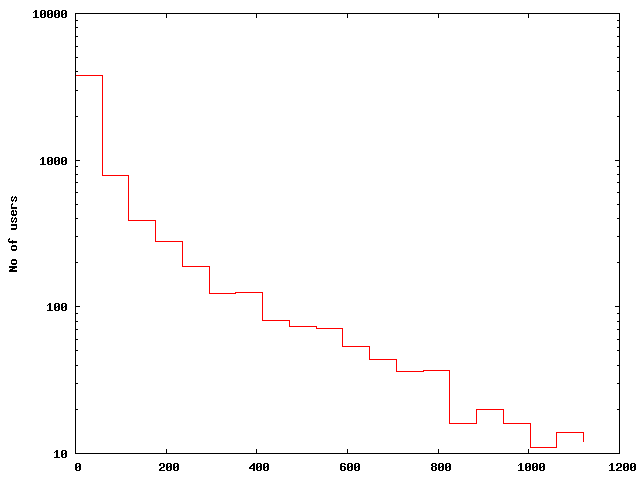
\includegraphics[scale=0.6]{images/favs.png}
		\label{fig:favs}
  }
  \subfigure[Subscriptions]{
		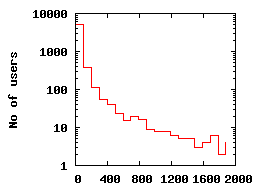
\includegraphics[scale=0.6]{images/subs.png}
		\label{fig:subs}
  }
  \subfigure[Uploads]{
		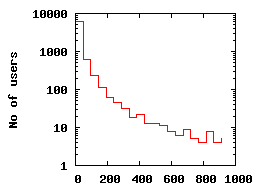
\includegraphics[scale=0.6]{images/ups.png}
		\label{fig:ups}
  }
  \label{fig:subfigureExample}
  \caption{Histograms of usage of favourites \subref{fig:favs}, subscriptions
  \subref{fig:subs} and uploads \subref{fig:ups}. The x axis represents groups of
  users having $x_1-x_2$ entities, the height of the bars indicates sizes of the
  groups.}
\end{figure}

\subsubsection{YouTube descriptions corpus}

A corpus of titles and descriptions for little over 100000 videos was collected
for text-based analysis of YouTube data. The file's size was 36 Mbytes. This
data was used to compute number of videos with identifiable concepts from
freebase data vocabularies.

\newpage
\subsection{Twitter}

Data available on \textit{Twitter} is composed of natural language short messages posted by users
consisting of up to 140 characters, commonly known as \textbf{tweets} \cite{why-we-twitter}. Within
those tweets we can distinguish user mentions (\textit{Twitter} usernames preceeded with the symbol \@,
such as \textit{@justinbieber}) as well as topics in form of `Hashtags` (name stripped of all whitespace
and preceded by the hash symbol -- e.g. \textit{\#TheDailyShow}) \cite{edinburg-corpus}.

The initial purpose of tweets was to inform other users of currently performed activities. However, as this service has
evolved, users started to use `tweets` for a variety of purposes, such as conversations, sharing information/URLs and reporting news(\cite{why-we-twitter} , \cite{twitter-content-is-it}). In order to use such unstructured data,
certain approaches need to be undertaken in order to extract information about their activities related to
the media. In this section we describe available methods to achieve this as well as measurements
that may be applied to the aggregated data. We will use the word \textit{entity} to refer to
known media people, shows and programmes.

Due to the structure of a regular \textit{Twitter} stream, certain ways of extracting references to entities
must be found. In our experiments, we focus on the following:

\paragraph{Mentioning entities' names}
Using trivial string matching methods, we search for entity names within \textit{Twitter} users' steams and updates.
mentions of entities' names in tweets. Multiple occurrences of entity names in the stream indicate interest
in the entity mentioned \cite{twitter-content-is-it} \\
Entities might be mentioned by:
\begin{itemize}
  \item \textit{full name}
  \item \textit{Hashtag}
  \item \textit{twitter username} - by entity's twitter username (if known)
  \item \textit{full name acronyms} - by acronyms built upon entity names
\end{itemize}
\paragraph{Usage of preference verbs when tweeting about entities}
In order to extract preference towards an entity from a tweet, a set of verbs
that express preference (both positive, such as \textit{enjoyed}, as well as negative \textit{hated})
was prepared. Those verbs were searched for in the tweets containing entity mentions.
\paragraph{Usage of activity verbs when tweeting about entities}
When mentioning a media-related entity, users may also describe the activity performed.
In order to find such tweets, an activity verbs vocabulary has also been prepared. Use of this vocabulary
might also decrease the chance of locating
Describing the activity of participating in a certain TV experience (such
as watching a show) will also need to be marked as due to the
fact that Twitter users are more likely to specify what they are doing at a
particular moment)
\paragraph{Extracting entities from structured twitter stream sources}
Applications, such as \textit{YouTube} or \textit{Boxee}\footnote[1]{http://www.boxee.tv}, automatically generate tweets
if the user linked their Twitter account with that application. These tweets are
usually well structured, and therefore very suitable to extract an entity, activity or preference.
\paragraph{Mentioning and following entities}
Mentions of entities followed (for known Twitter usernames) by the given user.

\begin{figure}[htp]
  \centering
  \begin{tabular}{ | p{4cm} | p{7cm} | } \hline
    \multicolumn{2}{|c|}{Types of measurements available} \\
    \hline
    \multirow{4}{*} {Mentioning entities}
      & Full name matching \\ \cline{2-2}
      & Matching the twitter username (if known) \\ \cline{2-2}
      & Matching name converted to a hashtag form \\
      & Matching the full name acronym \\ \cline{2-2}
    \hline
    Usage of activity verbs & Mentions using activity verbs \\
    \hline
    \multirow{3}{*}{Using preference verbs}
      & Mentions using preference verbs \\ \cline{2-2}
      & Positive preferences \\ \cline{2-2}
      & Negative preferences \\ \cline{2-2}
    \hline
    \multirow{3}{*}{Researching mentions}
      & Finding average amount of mentions-to-tweets ratio \\ \cline{2-2}
    \hline
  \end{tabular}
  \caption{Measures available for the Twitter tweets data corpus}
\end{figure}

\subsubsection{Corpus used for research}

The example data analyzed consists of Twitter streams consisting in total of about 50000 tweets. They have been selected from the followers of most popular TV channels and broadcasters available on Twitter basing on the amounts of tweets they have accumulated, the amount of their followers and the language they are tweeting in (English in this experiment).

The most significant reason for using a preselected corpus for this research is the Twitter API Rate Limiting
which makes a wider analysis challenging. Furthermore, a great deal of Twitter users provide completely irrelevant
information or tweet in languages barely useful for this research. All non-English mentions may be located,
but makes extracting preference information more challenging and decreases, which also
influences the effectiveness of a limited Twitter data aggregator. Using a preselected corpus enables measuring and comparing the effectiveness of different counting methods much easier. This idea has has been suggested by \cite{short-tweet} for
restricting the amount of subjects to be recommended, due to the high volume of tweets on \textit{Twitter}.
